The drones have essentially the same setup, but with slightly different configurations as they use different companion boards. This section describes the systems generally, referring to the specific companion boards only when necessary.

Figure \ref{fig:hardware_setup} shows a diagram of the hardware setup for the two drones. The components and their purposes are outlined below:
\begin{itemize}
    \item \textbf{11.1 V LiPo Battery:} this battery provides power to a battery eliminator circuit (BEC) for isolation of the power system for the computational electronics (the flight controller and companion board).
    \item \textbf{BEC (Battery Eliminator Circuit):} the BEC transforms 11.1V power to 5V power for the flight controller and companion board. The flight controller and companion board each have their own 4A channel to meet their given power requirements.
    \item \textbf{Flight Controller:} this combination of a Raspberry Pi 3 B+ and Navio2 shield runs the ArduPilot software to control the drone, and communicates with the companion board to control the gimbal.
    \item \textbf{Telemetry Radio:} the telemetry radio provides two-way communication between the flight controller and a ground control station that is also fitted with its own telemetry radio. It is connected to the flight controller via USB. The software on the ground control station provides an interface for real-time status messages and sending high-level commands.
    \item \textbf{RC Receiver:} the RC receiver provides a one-way radio link between the pilot's transmitter and the flight controller, allowing the pilot to manually control the drone. It is connected to the flight controller via SBus which provides an 8-channel multiplexed PWM signal to reduce the needed wires and space. This provides an interface for control by a human pilot, which is often used in testing but will eventually be mostly unused.
    \item \textbf{22.2 V LiPo Battery:} this battery provides power to the speed controllers and gimbal.
    \item \textbf{Speed Controllers:} the speed controllers receive a PWM signal from the flight controller which indicates a throttle value. They then provide corresponding power signals to the motors.
    \item \textbf{Motors:} the motors spin propellers to provide thrust in order to control the drone's position in the air.
    \item \textbf{Gimbal:} the gimbal controls the orientation of the camera based on PWM signals from the flight controller which indicate target angles. Its onboard IMU and driver filter the motion of the camera in order to provide a smooth camera image.
    \item \textbf{Companion Board:} the companion board reads an image from the camera and calculates the position of the landing pad relative to the drone. It then communicates this information to the flight controller via an Ethernet over USB connection using ROS.
    
\end{itemize}

\begin{figure}
    \centering
    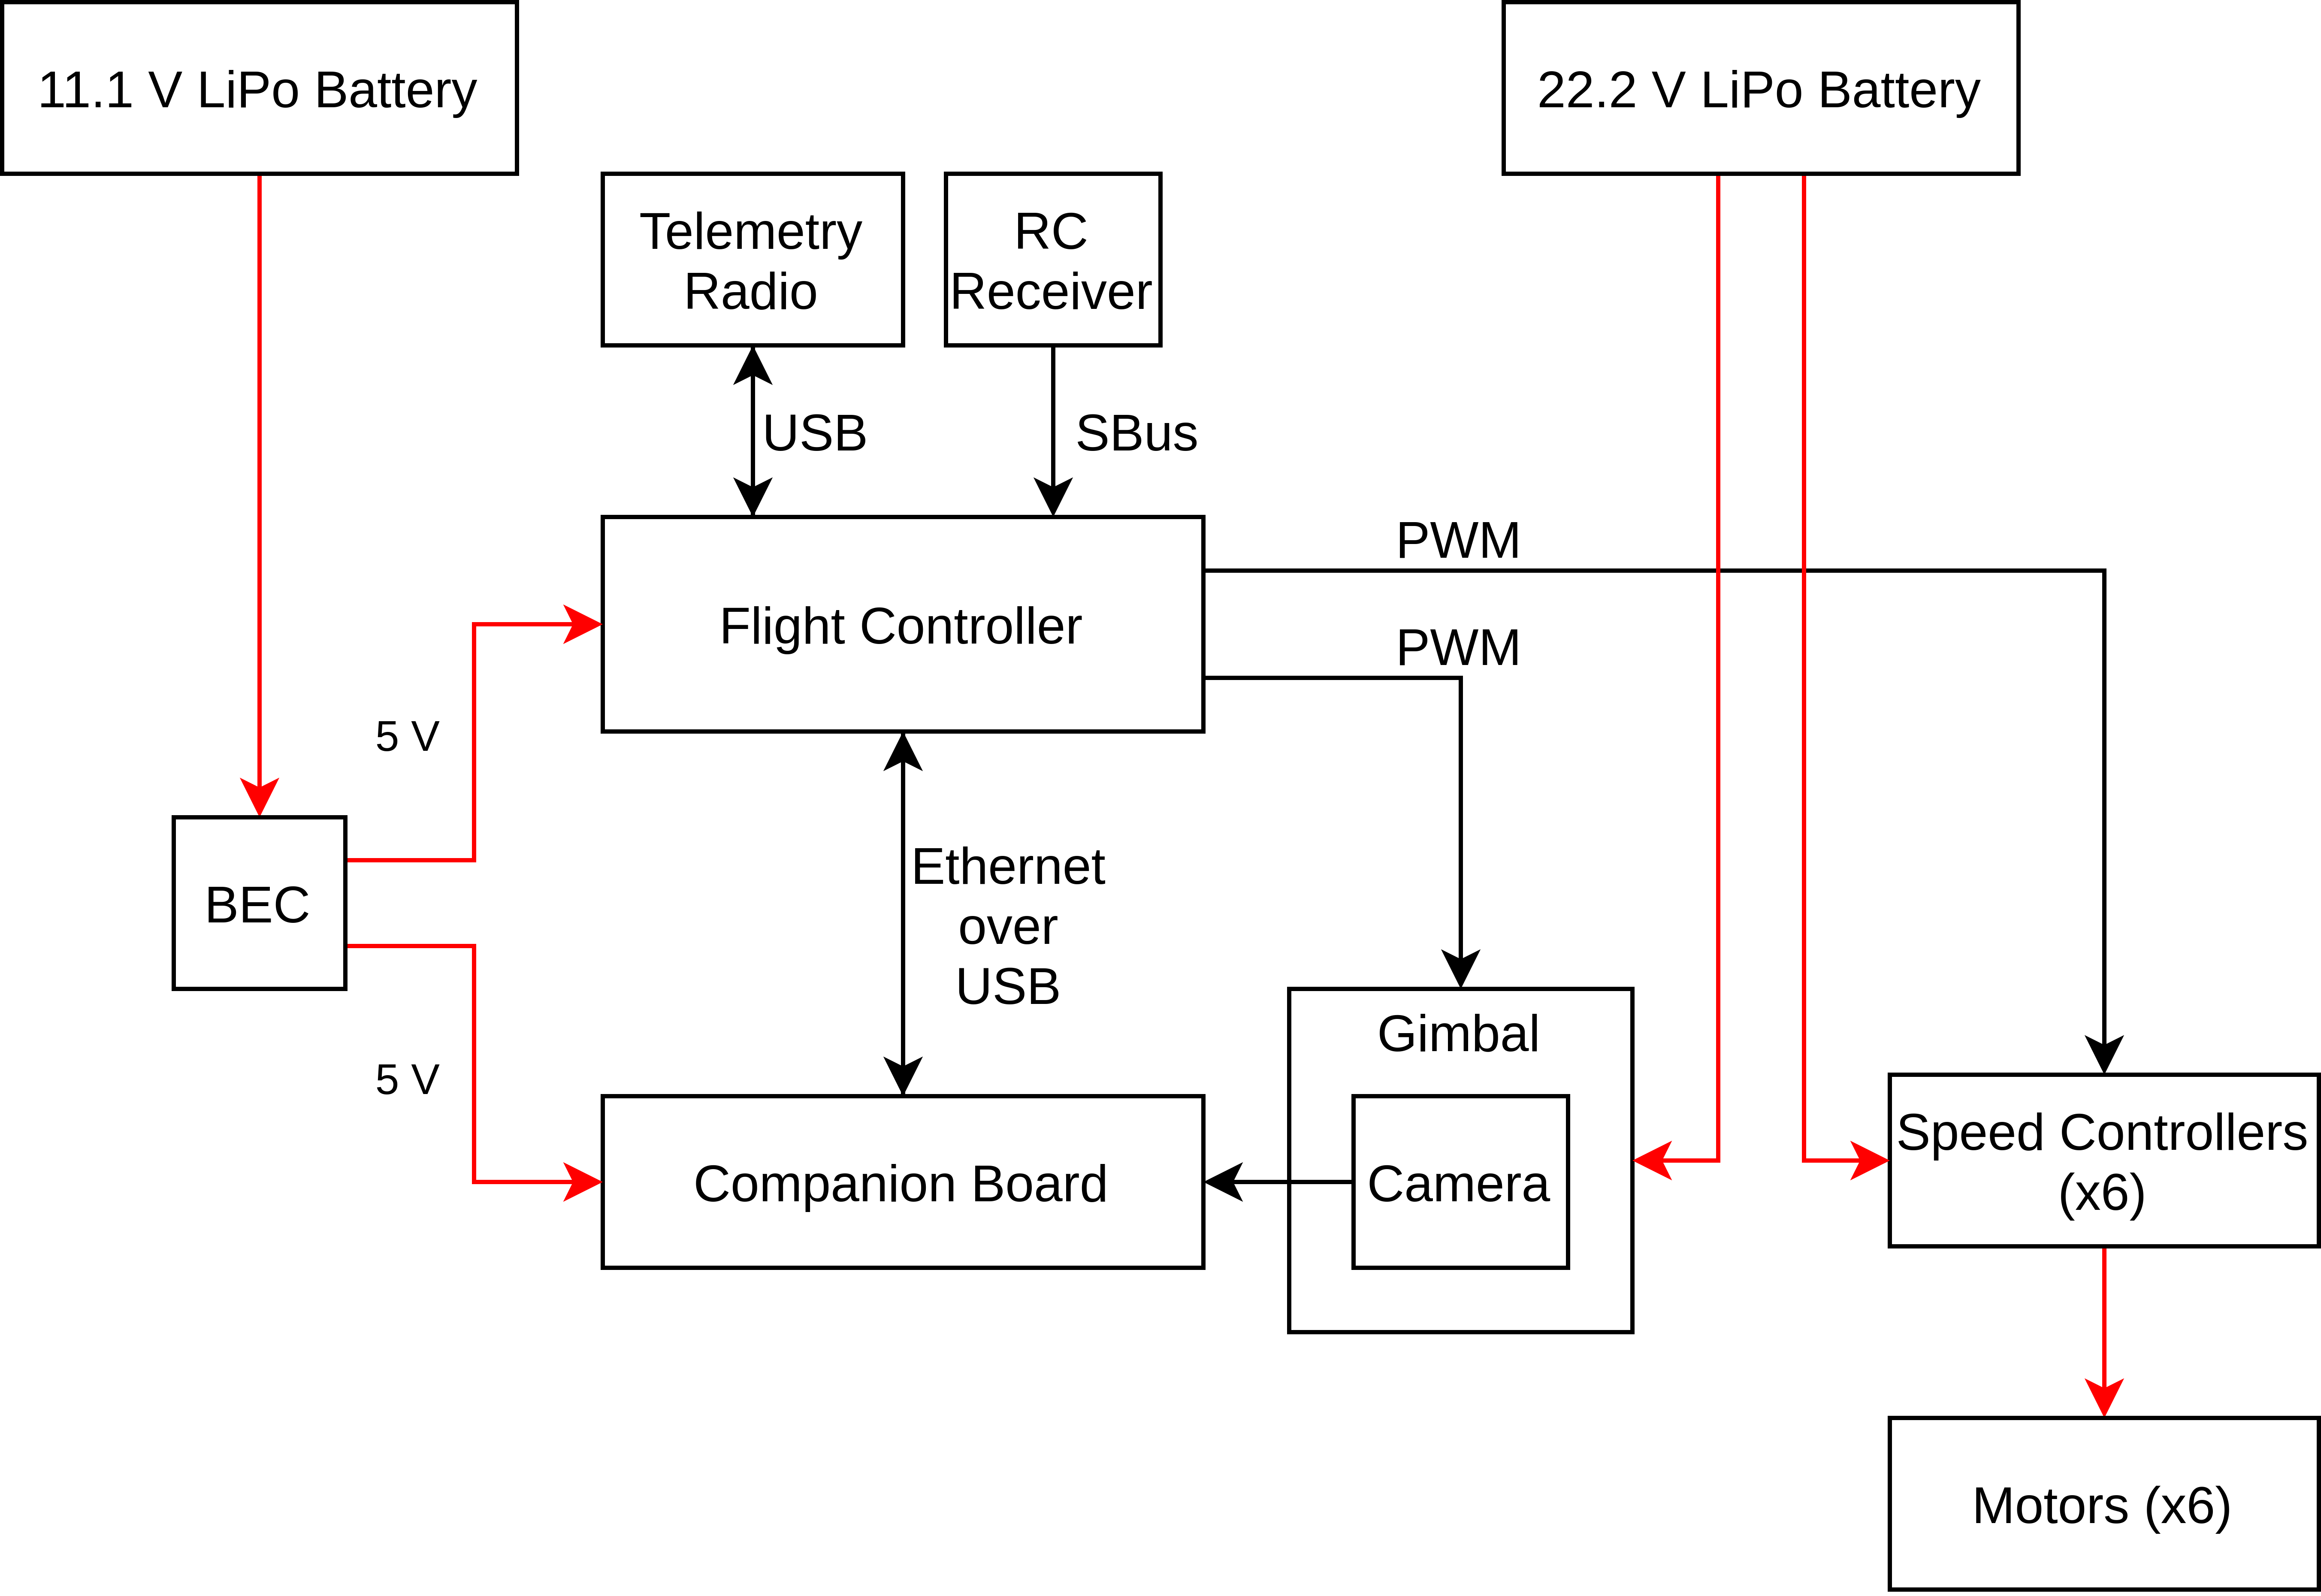
\includegraphics[width=0.8\textwidth]{images/hardware.png}
    \caption{Hardware Setup}
    \label{fig:hardware_setup}
\end{figure}

\subsection{Flight Controller Unit}

The flight controller unit (FCU) on both drones is a Raspberry Pi 3 B+ with a mounted Navio2 \cite{navio2_website} shield. The Navio2 provides inertial measurement data to the onboard autopilot software \textit{ArduPilot}, which is available open source \cite{ardupilot_website}. It runs as a system service in the Emlid distribution of the Raspbian OS, which is designed specifically for the Navio2. ArduPilot provides modes for manual, semi-autonomous, and fully autonomous flight. The ArduPilot software has \textit{not} been modified for this project. A ROS \cite{ros} module called MAVROS \cite{mavros} communicates with ArduPilot via its MAVLink \cite{mavlink_website} language in order to enable networked communication with the companion boards.

\subsection{Companion Boards}

Each drone has a second onboard processor (in addition to the flight controller), called a \textit{companion board}, the point of which is to reduce the computational load on the flight controller, which must run in real time. The companion board carries out the required video analysis, pose estimation, coordinate system transforms, and instantiates PID controllers to aim the gimbal. It then sends commands via MAVROS to the flight controller to act on this information. Connections between the companion board and the FCU are minimized in order to maintain modularity and decrease hardware and software invasiveness. Conveniently, each of the companion boards can act as a USB host, providing Ethernet over USB with static IP addresses on each end. This means that the only data connection between the companion board and the FCU is a single USB connection. Communication is established by configuring the ROS instance on the companion board to use a ROS Master instance on the FCU. This is accomplished simply by setting the \texttt{ROS\_MASTER\_URI} environment variable to the IP:port combination of the FCU, and setting the \texttt{ROS\_HOSTNAME} environment variable to the companion board's hostname. Initial setups accomplished this same configuration over a physical Ethernet connection, but the USB setup was proven more reliable given the space limitations in the drones' electronics compartments. (Physical pressure was put on the Ethernet cables when the canopy was closed, breaking the connection unpredictably.) Kjartan also tested a simulated Ethernet connection that was established from the Jetson Nano's UART port to the Raspberry Pi's USB port using two PPP services - one on the Raspberry Pi and one on the Jetson Nano. Acceptable connectivity between the boards when the services were configured to a baud rate of about 1,000,000. However, this was ultimately less reliable than using the Jetson Nano's native USB host functionality because of issues with the PPP services not syncing during boot. Using Ethernet over USB also eliminated the extra static IP configuration required with conventional Ethernet.

% An NVIDIA Jetson Nano is included on the drone in order to act as a companion board, reducing the computational requirements of the FCU. The Jetson Nano handles the image processing and coordinate system transformations that are involved in locating the landing pad via computer vision. It runs ROS modules (as system services) to carry out these tasks, and the ROS system is configured to act as a slave system to the ROS instance on the Raspberry Pi, via a single Ethernet connection. WhyCon and April Tag ROS modules analyze the image from the onboard camera to locate the fiducial markers on the landing pad. Proportional-integral-derivative (PID) controllers aim the camera directly at the markers by determining the markers' positions in the camera frame, attempting to place the markers in the center of the frame. The pan and tilt axes of the camera's gimbal are controlled by PWM signals generated by the Navio2, and the duty cycles of these signals are sent from the Jetson Nano to the Navio2, so that hardware connections from the companion board to the drone system are minimized. The channels for the gimbal tilt and pan are configured to forward the manual input signals from the drone operator to the PWM output rail, allowing the gimbal to be controlled manually during normal flight. However, when a fiducial marker is identified and the FCU is in ``Guided'' mode, this manual control is overridden using the MAVROS {\color{red} override RC in} topic. This has two principal benefits: first, the drone is able to switch between manual and automatic gimbal control, and second, the PWM connections to the gimbal are made on the FCU. This maintains modularity with respect to the companion board.

% Further, the WhyCon and April Tag ROS modules determine the positions of their respective fiducial markers in space. This allows the drone to identify and locate the landing pad, which is fitted with fiducial markers. These modules output the \textit{pose} (translation and rotation) of the fiducial markers with respect to the camera. The gimbal controller and landing controller ROS modules manipulate this pose to determine the pose of the camera with respect to the markers, and taking into considering the pan of the gimbal. Finally, three PID controllers use this information to calculate a target velocity that will direct the drone towards the landing pad. This target velocity is sent to the FCU and ArduPilot carries out all low-level commands to achieve this target velocity.

